\begin{name}
	{\tenchude}
	{\tendethi}
	{\tentruong}
	{\thoigian}
	\end{name}
\TN
\Opensolutionfile{ans}[ans/de5-phanI]
\begin{ex}%Câu 1
	Cho hàm số $y=f(x)$ có bảng biến thiên như sau
	\begin{center}
		
\begin{tikzpicture}
			\tkzTabInit[nocadre=false,lgt=1.2,espcl=2.5,deltacl=0.6]
			{$x$ /0.6,$y'$ /0.6,$y$ /2}
			{$-\infty$,$-1$,$0$,$1$,$+\infty$}
			\tkzTabLine{,-,$0$,+,$0$,-,$0$,+,}
			\tkzTabVar{+/$+\infty$, -/$1$,+/$2$,-/$1$,+/$+\infty$}
		\end{tikzpicture}
	\end{center}
	Hàm số đã cho nghịch biến trên khoảng nào dưới đây?
	\choice
	{$(0;+\infty)$}
	{$(-\infty;1)$}
	{\True $(0;1)$}
	{$(-1;0)$}
	\loigiai{
		Quan sát bảng biến thiên ta thấy $y'<0$ trên các khoảng $(-\infty;-1)$ và $(0;1)$ nên hàm số đã cho nghịch biến trên các khoảng $(-\infty;-1)$ và $(0;1)$.
	}
\end{ex}
\begin{ex}%Câu 2
	Họ tất cả các nguyên hàm của hàm số $f(x)=4x+\sin x$ là
	\choice
	{\True $2x^2-\cos x+C$}
	{$2x^2+\cos x+C$}
	{$2x^2-\sin x+C$}
	{$2x^2+\sin x+C$}
	\loigiai{
		Ta có 
		\begin{align*}
			\displaystyle \int f(x)\mathrm{\,d}x &= \int \left(4x+\sin x\right) \mathrm{\,d}x \\
			&= \int 4x\mathrm{\,d}x+\int \sin x \mathrm{\,d}x\\
			&=4\cdot \dfrac{x^2}{2}-\cos x+C\\
			&=2x^2-\cos x+C.
		\end{align*}
	}
\end{ex}
\begin{ex}%Câu 3
	Kết quả khảo sát cân nặng số táo ở lô hàng $B$ được cho ở bảng sau
	\begin{center}
		\begin{tabular}{|c|c|c|c|c|c|}
			\hline
			Cân nặng (g) & $[150;155)$ & $[155;160)$ & $[160;165)$ & $[165;170)$ & $[170;175)$ \\
			\hline
			Số quả táo ở lô hàng $B$ & $1$ & $3$ & $7$ & $10$ & $4$ \\
			\hline
		\end{tabular}
	\end{center}
	Số tạo được khảo sát trong bảng số liệu là
	\choice
	{$6$}
	{\True $25$}
	{$7$}
	{$5$}
	\loigiai{
		Số táo 	được khảo sát trong bảng số liệu là $n=1+3+7+10+4=25$.
	}
\end{ex}
\textbf{\textit{Sử dụng thông tin dưới đây để trả lời câu \ref{câu 4-đề 5} và câu \ref{câu 5-đề 5}}}\\[0.5em]
Trong không gian $Oxyz$, cho mặt phẳng $(P)\colon 2x-3y+6z-5=0$ và điểm $A(2;-3;1)$.
\begin{ex}%Câu 4
	\label{câu 4-đề 5}
	Một vectơ pháp tuyến của mặt phẳng $(P)$ là
	\choice
	{$\overrightarrow{n}_1=(2;-3;-5)$}
	{\True $\overrightarrow{n}_2=(2;-3;6)$}
	{$\overrightarrow{n}_3=(2;3;-5)$}
	{$\overrightarrow{n}_4=(2;-3;5)$}
	\loigiai{
		Một vectơ pháp tuyến của mặt phẳng $(P)$ là $\overrightarrow{n}=(2;-3;6)$.
	}
\end{ex}
\begin{ex}%Câu 5
	\label{câu 5-đề 5}
	Đường thẳng $d$ đi qua điểm $A$ và vuông góc với mặt phẳng $(P)$ có phương trình tham số là
	\choice
	{$d\colon\heva{& x=2+2t \\ & y=-3-3t\\ & z=1-5t}$}
	{$d\colon\heva{& x=2+2t \\ & y=-3-3t\\ & z=6+t}$}
	{\True $d\colon\heva{& x=2+2t \\ & y=-3-3t\\ & z=1+6t}$}
	{$d\colon\heva{& x=-2+2t \\ & y=3-3t\\ & z=-1+6t}$}
	\loigiai{
		Ta có đường thẳng $d\perp (P)$  nên có vectơ chỉ phương là $\overrightarrow{u}_d=\overrightarrow{n}_{(P)}=(2;-3;6)$.\\
		Đường thẳng $d$ đi qua $A$ và có vectơ chỉ phương là $\overrightarrow{u}_d==(2;-3;6)$ có phương trình tham số là
		\[\heva{&x=2+2t\\&y=-3-3t\\&z=1+6t.}\]
	}
\end{ex}
\begin{ex}%Câu 6
	$\lim\left(-3n^3+2n^2-5\right)$ bằng
	\choice
	{$-3$}
	{$-6$}
	{\True $-\infty$}
	{$+\infty$}
	\loigiai{
		Ta có $\lim \left(-3n^3+2n^2-5\right)= \lim n^3 \left(-3+\dfrac{2}{n}-\dfrac{5}{n^3}\right)$.\\
		Vì $
		\heva{&\lim n^3=+\infty\\&\lim\left(-3+\dfrac{2}{n}- \dfrac{5}{n^3}\right)=-3<0}$ nên  $\lim n^3 \left(-3+\dfrac{2}{n}-\dfrac{5}{n^3}\right)=-\infty$.\\ Suy ra $\lim \left(-3n^3+2n^2-5\right)=-\infty$ .
	}
\end{ex}
\begin{ex}%Câu 7
	\immini[thm]
	{
		Diện tích hình thang cong ở hình vẽ bên là $S=10$. Tích phân $\displaystyle\int\limits_{0}^{4} \left[4x+f(x)\right] \mathrm{\,d}x$ bằng
	\choice[2]
	{$14$}
	{\True $42$}
	{$32$}
	{$26$}
	}
	{
		\begin{tikzpicture}[scale=0.6,>=stealth, font=\footnotesize, line join=round, line cap=round]
			\def\a{0.25} \def\b{-1.5} \def\c{2.25} \def\d{2} % Hệ số
			\def\xmin{-1} \def\xmax{5}
			\def\ymin{-1} \def\ymax{4} 
			\draw[->] (\xmin,0)--(\xmax,0) node [below]{$x$};
			\draw[->] (0,\ymin)--(0,\ymax) node [left]{$y$};
			\node at (0,0) [below left]{$O$};
			\clip (\xmin+0.1,\ymin+0.1) rectangle (\xmax-0.5,\ymax-0.1);
			\draw[smooth,samples=300] plot(\x,{\a*(\x)^3+\b*(\x)^2+\c*(\x)+\d});
			\fill[pattern=north east lines,opacity=0.8] (0,0)--plot[domain=0:4](\x,{\a*(\x)^3+\b*(\x)^2+\c*(\x)+\d})--(4,0)--cycle;
			\draw[dashed] (4,0)node[below]{$4$}--(4,3) (0,2)node[left]{$2$};
		\end{tikzpicture}
	}
	\loigiai{
		Ta có $S=\displaystyle\int\limits_0^4 \left|f(x)\right|\mathrm{\,d}x=\displaystyle\int\limits_0^4 f(x)	\mathrm{\,d}x=10$.\\
		Do đó,
		\[
		\displaystyle\int\limits_0^4 \left[4x+f(x)\right]\mathrm{\,d}x=\displaystyle\int\limits_0^4 4x \mathrm{\,d}x+\displaystyle\int\limits_0^4 f(x)\mathrm{\,d}x
		=\left( 2x^2\right)\bigg|_0^4+10=32+10=42.
		\]
	}
\end{ex}
%\renewcommand{\baselinestretch}{1.4}
\begin{ex}%Câu 8
	Cho các số thực dương $a$, $b$ thỏa mãn $3\log a+2\log b=1$. Mệnh đề nào sau đây đúng?
	\choice
	{$a^3+b^2=1$}
	{$3a+2b=10$}
	{\True $a^3b^2=10$}
	{$a^3+b^2=10$}
	\loigiai{
		Ta có
		\[
		3\log a+2\log b=1\Leftrightarrow
		\log a^3+\log b^2 =1 \Leftrightarrow \log \left(a^3b^2\right) =1 \Leftrightarrow a^3b^2=10.
		\]
	}
\end{ex}
\begin{ex}%Câu 9
	Cho hình hộp $ABCD.A'B'C'D'$. Tính tổng $\overrightarrow{AB}+\overrightarrow{AD}+\overrightarrow{A'C'}$.
	\choice
	{$2\overrightarrow{AA'}$}
	{$\overrightarrow{0}$}
	{\True $2\overrightarrow{AC}$}
	{$2\overrightarrow{C'A'}$}
	\loigiai{
		Ta có $\overrightarrow{A'C'}=\overrightarrow{AC}$ và $\overrightarrow{AB}+\overrightarrow{AD}=\overrightarrow{AC}$ (quy tắc hình bình hành).\\
		Suy ra $\overrightarrow{AB}+\overrightarrow{AD}+\overrightarrow{A' C'}=\left(\overrightarrow{AB}+\overrightarrow{AD}\right)+\overrightarrow{A' C'}=\overrightarrow{AC}+\overrightarrow{AC}=2\overrightarrow{AC}$.
	}
\end{ex}
\begin{ex}%Câu 10
	Đồ thị hàm số $y=x^3-3x^2+2$ là đường cong nào trong hình sau đây?
	\choice
	{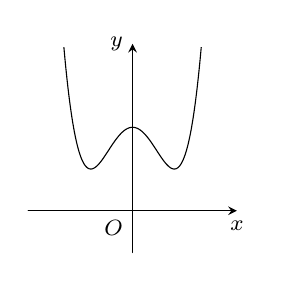
\begin{tikzpicture}[scale=0.53,>=stealth, font=\footnotesize, line join=round, line cap=round]
			\def\a{1} \def\b{-2} \def\c{2} % Hệ số
			\def\xmin{-2.5} \def\xmax{2.5}
			\def\ymin{-1} \def\ymax{4} 
			\draw[->] (\xmin,0)--(\xmax,0) node [below]{$x$};
			\draw[->] (0,\ymin)--(0,\ymax) node [left]{$y$};
			\node at (0,0) [below left]{$O$};
			\clip (\xmin+0.1,\ymin+0.1) rectangle (\xmax-0.5,\ymax-0.1);
			\draw[smooth,samples=300,domain=\xmin:\xmax] plot(\x,{\a*(\x)^4+\b*(\x)^2+\c});
	\end{tikzpicture}}
	{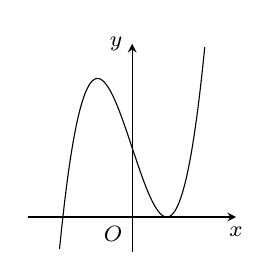
\begin{tikzpicture}[scale=0.44,>=stealth, font=\footnotesize, line join=round, line cap=round]
			\def\a{1} \def\b{0} \def\c{-3} \def\d{2} % Hệ số
			\def\xmin{-3} \def\xmax{3}
			\def\ymin{-1} \def\ymax{5} 
			\draw[->] (\xmin,0)--(\xmax,0) node [below]{$x$};
			\draw[->] (0,\ymin)--(0,\ymax) node [left]{$y$};
			\node at (0,0) [below left]{$O$};
			\clip (\xmin+0.1,\ymin+0.1) rectangle (\xmax-0.5,\ymax-0.1);
			\draw[smooth,samples=300] plot(\x,{\a*(\x)^3+\b*(\x)^2+\c*(\x)+\d});
	\end{tikzpicture}}
	{\True 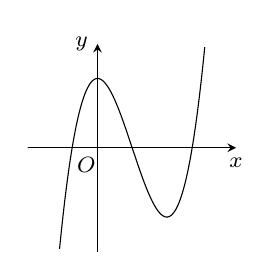
\begin{tikzpicture}[scale=0.44,>=stealth, font=\footnotesize, line join=round, line cap=round]
			\def\a{1} \def\b{-3} \def\c{0} \def\d{2} % Hệ số
			\def\xmin{-2} \def\xmax{4}
			\def\ymin{-3} \def\ymax{3} 
			\draw[->] (\xmin,0)--(\xmax,0) node [below]{$x$};
			\draw[->] (0,\ymin)--(0,\ymax) node [left]{$y$};
			\node at (0,0) [below left,xshift=0.1cm]{$O$};
			\clip (\xmin+0.1,\ymin+0.1) rectangle (\xmax-0.5,\ymax-0.1);
			\draw[smooth,samples=300] plot(\x,{\a*(\x)^3+\b*(\x)^2+\c*(\x)+\d});
	\end{tikzpicture}}
	{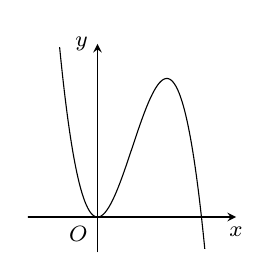
\begin{tikzpicture}[scale=0.44,>=stealth, font=\footnotesize, line join=round, line cap=round]
			\def\a{-1} \def\b{3} \def\c{0} \def\d{0} % Hệ số
			\def\xmin{-2} \def\xmax{4}
			\def\ymin{-1} \def\ymax{5} 
			\draw[->] (\xmin,0)--(\xmax,0) node [below]{$x$};
			\draw[->] (0,\ymin)--(0,\ymax) node [left]{$y$};
			\node at (0,0) [below left]{$O$};
			\clip (\xmin+0.1,\ymin+0.1) rectangle (\xmax-0.5,\ymax-0.1);
			\draw[smooth,samples=300] plot(\x,{\a*(\x)^3+\b*(\x)^2+\c*(\x)+\d});
	\end{tikzpicture}}
	\loigiai{
		Đồ thị hàm bậc ba $y=x^3-3x^2+2$ với $a>0$ nên loại 
		\begin{center}
			\begin{tabular}{cc}
				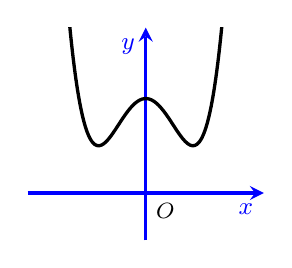
\begin{tikzpicture}[thick,>=stealth,scale=0.6] 
					\clip(-2.5,-1) rectangle (2.5,3.5);
					\draw[->,very thick,blue] (-2.5,0) -- (2.5,0) node[below left] {\small $x$};
					\draw[->,very thick,blue] (0,-1) -- (0,3.5) node[below left] {\small $y$};
					\draw [fill=white,draw=blue] (0,0) circle (1pt)node[below right] {\footnotesize $O$};
					\draw[very thick,black,smooth,samples=100,domain=-2.5:2.5] plot(\x,{(\x)^4-2*(\x)^2+2});
					%	\draw[dashed, thick,blue] 
					%	(1,0) node[below]{1}|-(0,1) node[above left]{1}
					%	(-1,0) node[below]{-1}|-(0,1)node[left]{};
				\end{tikzpicture}
				&
				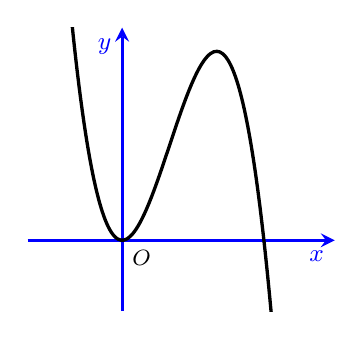
\begin{tikzpicture}[thick,>=stealth,scale=0.6] 
					\clip(-2,-1.5) rectangle (4.5,4.5);
					\draw[->,very thick,blue] (-2,0) -- (4.5,0) node[below left] {\small $x$};
					\draw[->,very thick,blue] (0,-1.5) -- (0,4.5) node[below left] {\small $y$};
					\draw [fill=white,draw=blue] (0,0) circle (1pt)node[below right] {\footnotesize $O$};
					\draw[very thick,black,smooth,samples=100,domain=-2:4.5] plot(\x,{-(\x)^3+3*(\x)^2});
					%	\draw[dashed, thick,blue] 
					%	(1,0) node[below]{1}|-(0,1) node[above left]{1}
					%	(-1,0) node[below]{-1}|-(0,1)node[left]{};
				\end{tikzpicture}
			\end{tabular}
		\end{center}
		Hàm số $y=x^3-3x^2+2$ có $y'=3x^2-6x$. Cho $y'=0 \Rightarrow \hoac{&x=0\\&x=2.}$\\
		Suy ra $x=0$ và $x=2$ là hai điểm cực trị nên chọn
		\begin{center}
			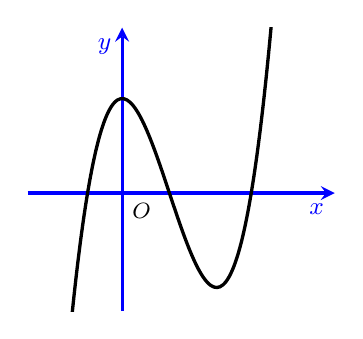
\begin{tikzpicture}[thick,>=stealth,scale=0.6] 
				\clip(-2,-2.5) rectangle (4.5,3.5);
				\draw[->,very thick,blue] (-2,0) -- (4.5,0) node[below left] {\small $x$};
				\draw[->,very thick,blue] (0,-2.5) -- (0,3.5) node[below left] {\small $y$};
				\draw [fill=white,draw=blue] (0,0) circle (1pt)node[below right] {\footnotesize $O$};
				\draw[very thick,black,smooth,samples=100,domain=-2:4.5] plot(\x,{(\x)^3-3*(\x)^2+2});
			\end{tikzpicture}
		\end{center}
	}
\end{ex}
\begin{ex}%Câu 11
	Cho hình chóp $S.ABCD$ có đáy $ABCD$ là hình thoi tâm $O$. Biết rằng $SA=SC$ và $SB=SD$. Khẳng định nào sau đây là \textbf{sai}?
	\choice
	{$SO\perp(ABCD)$}
	{$AC\perp BD$}
	{$(SBD)\perp(SAC)$}
	{\True $BD\perp SD$}
	\loigiai{
		\immini{
			Ta có $\heva{& SO\perp AC\\& SO\perp BD}\Rightarrow SO\perp (ABCD)$ đúng.\\
			Vì $ABCD$ là hình thoi nên $AC\perp BD$ đúng.\\
			Ta có $\heva{& BD\perp AC\\& BD\perp SO} \Rightarrow BD\perp (SAC)$
			Suy ra $\heva{& BD\subset (SBD)\\& BD\perp (SAC)}\Rightarrow (SBD)\perp (SAC)
			$ đúng.\\
			Ta có $BD\subset (SBD)$ mà tam giác $SBD$ cân tại $S$ nên $\widehat{SDB}=\widehat{SBD}<90^\circ$ do đó $BD\perp SD$ sai.
		}{
			\begin{tikzpicture}[declare function={a=2;b=4;h=4;},line join=round]
				\path (0,0) coordinate (A)
				(-145:a) coordinate (B)
				(b,0) coordinate (D)
				($ (B)!0.5!(D) $) coordinate (O)
				($(O)+(0,h) $) coordinate (S);
				\path ($(D)-(A)+(B)$) coordinate (C);
				\draw[dashed] (S)--(A)--(B) (A)--(D)--(B) (A)--(C) (S)--(O);
				\draw (B)--(C)--(D) (B)--(S)  (D)--(S)--(C);
				\foreach \x/\y/\z in {S/O/B,S/O/C,A/O/B}{
					\path pic[draw,angle radius=5pt]{right angle= \x--\y--\z};
				}
				\foreach \t/\g in {A/150,B/-90,C/-90,D/0,S/90,O/-90}{
					\draw[fill=black] (\t) circle (1pt) node[shift={(\g:7pt)},font=\scriptsize]{$ \t $};
				}
			\end{tikzpicture}
		}
	}
\end{ex}
\begin{ex}%Câu 12
	Tìm tập nghiệm $S$ của bất phương trình $\log_{\tfrac{1}{5}}\left(x^2-1\right)<\log_{\tfrac{1}{5}}\left(3x-3\right)$.
	\choice
	{\True $S=(2;+\infty)$}
	{$S=(-\infty;1)\cup(2;+\infty)$}
	{$S=(-\infty;-1)\cup(2;+\infty)$}
	{$S=(1;2)$}
	\loigiai{
		Phương trình đã cho tương đương
		\[
		\heva{&x^2-1>3x-3\\&3x-3>0}\Leftrightarrow \heva{&x^2-3x+2>0\\&x>1} \Leftrightarrow \heva{&\hoac{&x<1\\&x>2}\\&x>1} \Leftrightarrow x>2.
		\]
		Vậy tập nghiệm của bất phương trình là $S=(2;+\infty)$.
	}
\end{ex}
\Closesolutionfile{ans}
%{\fontfamily{qtm}\fontsize{13pt}{2pt}\selectfont\textbf{PHẦN II. Câu trắc nghiệm đúng sai}. Thí sinh trả lời từ câu 1 đến câu 4. Trong mỗi ý \textbf{a)}, \textbf{b)}, \textbf{c)}, \textbf{d)} ở mỗi câu, thí sinh chọn đúng hoặc sai.}
%\setcounter{ex}{0}% Reset lại số đếm câu hỏi
\TNTF
\Opensolutionfile{ans}[ans/de5-phanII]
\begin{ex}%Câu 1
	Trong không gian $Oxyz$, cho các điểm $A(0;-1;1)$, $B(-2;1;-1)$ và $C$ thỏa mãn điều kiện $\overrightarrow{OC}=-\overrightarrow{i}+3\overrightarrow{j}+2\overrightarrow{k}$. Xét tính đúng sai của các mệnh đề sau
	\choiceTF
	{Tọa độ điểm $C$ là $(-1;2;3)$}
	{\True Tọa độ các vectơ $\overrightarrow{AB}=(-2;2;-2)$ và $\overrightarrow{AC}=(-1;4;1)$}
	{Một vectơ pháp tuyến của mặt phẳng $(ABC)$ là $(5;-2;-3)$}
	{Khoảng cách từ gốc tọa độ $O$ đến mặt phẳng $(ABC)$ bằng $\dfrac{5}{\sqrt{33}}$}
		\loigiai{
		\begin{itemchoice}
			\itemch 	Ta có $\overrightarrow{OC}=-\overrightarrow{i}+3\overrightarrow{j}+2\overrightarrow{k}$ nên tọa độ điểm $C(-1;3;2)$.
			\itemch Tọa độ $\overrightarrow{AB}=(-2;2;-2)$ và $\overrightarrow{AC}=(-1;4;1)$.
			\itemch 	Một vectơ pháp tuyến của mặt phẳng $(ABC)$ là \[\overrightarrow{n}=[\overrightarrow{AB},\overrightarrow{AC}] = (10;4;-6)=2(5;2;-3).\]
			\itemch Phương trình mặt phẳng $(ABC)$ là
			\[
			5(x-0)+2(y+1)-3(z-1)=0 \Leftrightarrow 5x+2y-3z+5=0.
			\]
			Khoảng cách từ $O$ đến $(ABC)$ là
			\[
			\mathrm{d}(O,(ABC))=\dfrac{|5\cdot 0+2\cdot 0-3\cdot 0+5|}{\sqrt{5^2+2^2+(-3)^2}}=\dfrac{5}{\sqrt{38}}=\dfrac{5\sqrt{38}}{38}.
			\]
		\end{itemchoice}	
	}
\end{ex}
\begin{ex}%Câu 2
	Tốc độ giao đổi chất cơ bản của sinh vật có thể tăng hoặc giảm tùy thuộc vòa hoạt động của sinh vật. Cụ thể sau khi hấp thụ chất dinh dưỡng, sinh vật thường trải qua một sự tăng đột biến trong tốc độ trao đổi chất của nó, sau đó dần dần trở lại mức cơ bản. Linh vừa kết thúc bữa ăn tối của mình với năng lượng nạp vào là $5120$ J và tốc độ trao đổi chất của cô đã tăng đột biến từ mức cơ bản $M_0$. Sau đó cô đã tiêu hao hết năng lượng đó trong $12$ giờ tiếp theo. Giả sử $t$ giờ sau bữa ăn Linh tiêu hao được $M(t)$ kJ, tốc độ trao đổi chất của cô được cho bởi hàm số $M'(t)=M_0+t\mathrm{e}^{-0{,}1t^2}$ (kJ/h), $t\in[0;12]$. Xét tính đúng sai của các mệnh đề sau
	\choiceTF
	{\True $M(t)=M_0t-5\mathrm{e}^{-0{,}1t^2}+C$ là họ nguyên hàm của hàm số $M'(t)$}
	{\True $M_0=0{,}01$ (làm tròn đến hàng phần trăm)}
	{\True Năng lượng còn lại sau $6$ giờ đâu là $197$ J (làm tròn đến hàng đơn vị)}
	{Tốc độ tiêu hao năng lượng trung bình trong khoảng thời gian từ $a$ giờ tới $b$ giờ được tính bởi công thức $v_{\text{tb}}=\dfrac{M(b)-M(a)}{b-a}$. Tốc độ tiêu hao năng lượng trung bình từ $6$ giờ đến $12$ giờ của Linh là $32{,}76$ J/h (làm tròn kết quả đến hàng đơn vị)}
	\loigiai{
		\begin{itemchoice}
			\itemch Ta có $M'(t)=\left(M_0 t-5\mathrm{e}^{-0{,}1t^2}+C\right)' = M_0+t\mathrm{e}^{-0{,}1t^2}$.\\
			Suy ra $\displaystyle \int M'(t)\mathrm{\,d}t=M(t)=M_0 t-5\mathrm{e}^{-0{,}1t^2}+C$.
			\itemch Tổng năng lượng tiêu hao trong khoảng thời gian $12$ giờ là $5\,120$ J $ =5{,}12$ kJ tức là
			\[
			M(12)-M(0)=5{,}12\,\,\text{kJ}.
			\]
			Khi $t=12$ ta có $M(12)=M_0\cdot 12-5\mathrm{e}^{-0{,}1\cdot 12^2}+C$.\\
			Khi $t=0$ ta có $M(0)=M_0\cdot 0-5\mathrm{e}^{-0{,}1\cdot 0^2}+C=-5+C$.\\
			Suy ra $M(12)-M(0)=12M_0-5\left( \mathrm{e}^{-0{,}1\cdot 12^2}-1\right)$.\\
			Thay $M(12)-M(0)=5\,120$ ta được
			\[
			12M_0-5\left( \mathrm{e}^{-0{,}1\cdot 12^2}-1\right) = 5{,}12
			\Leftrightarrow M_0=0{,}01\,\, \rm{kJ/h}.
			\]
			\itemch Năng lượng tiêu hao trong $6$ giờ
			\[
			M(6)-M(0)=6M_0-5\left(\mathrm{e}^{-0{,}1\cdot 6^2}-1\right)\approx 4{,}92\,\,\text{kJ}.
			\]
			Năng lượng còn lại sau $6$ giờ
			\[
			5120\,\,\text{J}-4920\,\,\text{J}=200\,\,{J}.
			\]
			\itemch 	Tốc độ tiêu hao trung bình từ $6$ giờ đến $12$ giờ là
			\[
			v_{\text{tb}}=\dfrac{M(12)-M(6)}{12-6}=\dfrac{6M_0-5\left(\mathrm{e}^{-0{,}1\cdot 12^2}-\mathrm{e}^{-0{,}1\cdot 6^2}\right)}{6}\approx 0{,}0327695\,\,\rm{kJ/h}\approx 32{,}77 \,\,\rm{J/h}.
			\]
		\end{itemchoice}	
	}
\end{ex}
%\renewcommand{\baselinestretch}{1.4}
\begin{ex}%Câu 3
	\immini[thm]
	{
		Ta có Trái Đất là hình cầu hoàn hảo với bán kính $R=6370$ km và diện tích toàn phần là $S=4\pi R^2$. Các phi hành gia từ tàu vũ trụ chỉ có thể nhìn thấy một phần bề mặt Trái Đất. Ở độ cao $h$, phần diện tích Trái Đất các phi hành gia có thể nhìn thấy sẽ được tính theo công thức $S_{T}=2\pi R^2\left(1-\dfrac{R}{R+h}\right)$, trong đó $R$ là bán kính Trái Đất. Gọi $K$ là tỷ số diện tích bề mặt Trái Đất nhìn thấy được ở độ cao $h$ với diện tích toàn phần của Trái Đất. Xét tính đúng sai của các mệnh đề sau
	}
	{
		\begin{tikzpicture}[scale=0.7,>=stealth, font=\footnotesize, line join=round, line cap=round]
			\coordinate (O) at (0,0);
			\draw (O)node[opacity=0.85]{\includegraphics[width=3.45cm]{images/de5-2}};
			\coordinate (M) at ($(O)+(-130:1.5cm)$);
			\coordinate (A) at (120:3 cm and 3 cm);
			\draw[dashed] (A) arc (120:-120:3 cm and 3 cm);
			\coordinate (A') at (0:3 cm and 3 cm);
			\draw (A')node[rotate=90,left,xshift=0.1cm]{\includegraphics[width=0.6cm]{images/de5-1}};
			\draw[dashed] (O)--(A') ($(O)!0.7!(A')$)node[above]{$h$};
			\coordinate (B) at (45:4.5 cm and 4.5 cm);
			\draw[dashed] (B) arc (45:-45:4.5 cm and 4.5 cm);
			\coordinate (B') at (0:4.5 cm and 4.5 cm);
			\draw (B')node[rotate=90,left,xshift=0.1cm]{\includegraphics[width=0.6cm]{images/de5-1}};
			\draw[thick] (O)--(M);
			\tkzDefLine[tangent from = A'](O,M)% with 4.25
			\tkzGetPoints{X}{Y} 
			\draw (A')--($(A')!1.5!(X)$) (A')--($(A')!1.5!(Y)$);
			\tkzDefLine[tangent from = B'](O,M)% with 4.25
			\tkzGetPoints{X'}{Y'}
			\draw[dashed] (B')--(X') (B')--(Y');
		\end{tikzpicture}
	}\vspace{3pt}
	\choiceTF
	{Công thức tính $K$ là $K=\dfrac{1}{2}\left(1-\dfrac{h}{R+h}\right)$}
	{Trong một chuyến bay của tàu con thoi, các phi hành gia đã thực hiện một hoạt động ngoài tàu ở độ cao $280$ km. Có $2{,}5\%$ (làm tròn đến hàng phần mười) diện tích bề mặt Trái Đất có thể nhìn thấy ở độ cao đó}
	{Muốn nhìn thấy $\dfrac{1}{4}$ diện tích bề mặt Trái Đất, các phi hành gia cần đưa tàu con thoi đạt đến độ cao $6470$ km}
	{\True Khi độ cao $h$ càng tăng lên thì $K$ càng tăng nhưng không vượt quá $50\%$}
	\loigiai{
		\begin{itemchoice}
			\itemch 	Ta có tỷ số $K$ là diện tích nhìn thấy được chia cho diện tích toàn phần
			\[
			K =\dfrac{S_T}{S}=\dfrac{2\pi R^2\left(1-\dfrac{R}{R+h}\right)}{4\pi R^2}
			= \dfrac{1}{2}\left(1-\dfrac{R}{R+h}\right)=\dfrac{1}{2}\cdot \dfrac{h}{R+h}.
			\]
			\itemch Với bán kính $R=6\,370$ km và chiều cao $h=280$ km thì tỷ số $K$ tại độ cao $h$ là
			\[
			K=\dfrac{1}{2}\cdot \dfrac{h}{R+h}=\dfrac{1}{2}\cdot \dfrac{280}{6\,370+280}=\dfrac{2}{95}\approx0{,}021\approx 2{,}1\%.
			\]		
			\itemch Với $K=\dfrac{1}{4}$ thì
			\[
			K=\dfrac{1}{2}\cdot \dfrac{h}{R+h}\Leftrightarrow \dfrac{1}{4}=\dfrac{1}{2}\cdot \dfrac{h}{6\,370+h}\Leftrightarrow h=6\,370\,\,\rm{(km)}.\]
			\itemch 	Khi $h$ càng lớn ta có
			\[
			\lim\limits_{h\rightarrow +\infty} K =\lim\limits_{h\rightarrow +\infty} \dfrac{1}{2}\dfrac{h}{R+h}=\dfrac{1}{2}\lim\limits_{h\rightarrow +\infty} \dfrac{1}{\dfrac{R}{h}+1}=\dfrac{1}{2}=0{,}5=50\%.
			\]
		\end{itemchoice}
	}
\end{ex}
\begin{ex}%Câu 4
	Ở một khu rừng nọ có $7$ chú lùn, trong đó có $5$ chú luôn nói thật, $2$ chú còn lại nói thật với xác suất $0{,}5$. Nàng Bạch Tuyết lạc vào trong rừng và gặp một chú lùn.
	\begin{itemize}
		\item Gọi $A$ là biến cố \lq\lq Chú lùn gặp được luôn nói thật\rq\rq.
		\item Gọi $B$ là biến cố \lq\lq Chú lùn đó tự nhận mình luôn nói thật\rq\rq.
	\end{itemize}
	Xét tính đúng sai của các mệnh đề sau\vspace{5pt}
	\choiceTF
	{\True $\mathrm{P}(A)=\dfrac{5}{7}$ và $\mathrm{P}(\overline{A})=\dfrac{2}{7}$}
	{Xác suất có điều kiện $\mathrm{P}(B\mid A)=0{,}5$}
	{\True $\mathrm{P}(B)=\dfrac{6}{7}$}
	{\True Nàng Bạch Tuyết gặp ngẫu nhiên một chú lùn. Biết rằng chú lùn mà Bạch Tuyết gặp tự nhận mình là luôn nói thật. Xác suất để chú lùn đó luôn nói thật là $\dfrac{5}{6}$}
	\loigiai{
		\begin{itemchoice}
			\itemch Ta có $\mathrm{P}(A)=\dfrac{5}{7}\Rightarrow \mathrm{P}(\overline{A}) = \dfrac{2}{7}$ 
			\itemch Xác xuất có điều kiện $P(B\mid A)=1$.
			\itemch Theo công thức Bayes, ta có
			\[\mathrm{P}(B)=\mathrm{P}(A) \cdot \mathrm{P}(B|A)+\mathrm{P}(\overline{A})\cdot\mathrm{P}(B|\overline{A}) \Leftrightarrow \mathrm{P}(B)=1\cdot \dfrac{5}{7}+ 0{,}5\cdot \dfrac{2}{7}=\dfrac{6}{7}.\]
			\itemch Ta có
			\[\mathrm{P}(A|B)=\dfrac{\mathrm{P}(AB)}{\mathrm{P(B)}}=\dfrac{\mathrm{P}(A)\cdot \mathrm{P}(B|A)}{\mathrm{P}(B)}= \dfrac{\dfrac{5}{7}\cdot 1}{\dfrac{6}{7}}=\dfrac{5}{6}.\]
		\end{itemchoice}	
	}
\end{ex}
\Closesolutionfile{ans}
%{\fontfamily{qtm}\fontsize{13pt}{2pt}\selectfont\textbf{PHẦN III. Câu trắc nghiệm trả lời ngắn}. Thí sinh trả lời từ câu 1 đến câu 6 và điền đáp án vào ô trống.}
%\setcounter{ex}{0}% Reset lại số đếm câu hỏi
\TNSA
\Opensolutionfile{ans}[ans/de5-phanIII]
\begin{ex}%Câu 1
	Cho hình chóp đều $S.ABCD$ có cạnh đáy bằng $4$, khoảng cách giữa hai đường thẳng $SA$ và $CD$ bằng $2$. Thể tích của khối chóp $S.ABCD$ bằng bao nhiêu? (làm tròn kết quả đến hàng phần mười).
	
	\shortans[0]{$6{,}2$}
	\loigiai{
		\immini{
			Diện tích mặt đáy $S_{ABCD}=4^2=16$.\\
			Chọn $(SAB)$ chứa $SA$, ta có $\heva{
				&CD\parallel AB\\
				&AB\subset (SAB).
			}$\\
			Suy ra $CD\parallel (SAB)$ nên 
			\begin{align*}
				\mathrm{d}(CD,SA)&=\mathrm{d}(CD,(SAB))=\mathrm{d}(D,(SAB))\\
				&=2\mathrm{d}(O,(SAB))=2\\
				\Rightarrow &\mathrm{d}(O,(SAB))=1.
			\end{align*}
			Gọi $H$ là hình chiếu vuông góc của $O$ trên $AB$ và 
		}{
			\begin{tikzpicture}[declare function={a=2;b=4;h=4;},line join=round]
				\path (0,0) coordinate (A)
				(-145:a) coordinate (B)
				(b,0) coordinate (D)
				($ (B)!0.5!(D) $) coordinate (O)
				($(O)+(0,h) $) coordinate (S);
				\path ($(D)-(A)+(B)$) coordinate (C);
				\path ($(A)!0.5!(B)$) coordinate (H);
				\path ($(S)!0.7! (H)$) coordinate (K);
				\draw[dashed] (S)--(A)--(B) (A)--(D)--(B) (A)--(C) (S)--(O)--(H)--(S) (K)--(O)--(H);
				\draw (B)--(C)--(D) (B)--(S)  (D)--(S)--(C);		
				\foreach \x/\y/\z in {S/O/B,S/O/C,A/O/B,O/H/A,O/K/S}{
					\path pic[draw,angle radius=5pt]{right angle= \x--\y--\z};
				}
				\foreach \t/\g in {A/160,B/-90,C/-90,D/0,S/90,O/-90,H/160,K/-140}{
					\draw[fill=black] (\t) circle (1pt) node[shift={(\g:7pt)},font=\scriptsize]{$ \t $};
				}
			\end{tikzpicture}
		}
		$K$ là hình chiếu vuông góc của $O$ trên $SH$, ta có
		\[
		\heva{
			&AB\perp OH\\
			&AB\perp SO
		}\Rightarrow AB\perp (SOH)\Rightarrow AB\perp OK.\quad (1)
		\]
		Mà $OK\perp SH$. \quad (2)\\
		Suy ra $OK\perp (SAB)\Rightarrow \mathrm{d}(O,(SAB))=OK=1$.\\
		Với $OH=\dfrac{1}{2}AD=2$ ta có
		\[
		\dfrac{1}{OK^2}=\dfrac{1}{OH^2}+\dfrac{1}{SO^2}\Leftrightarrow
		\dfrac{1}{SO^2}=\dfrac{1}{1^2}-\dfrac{1}{2^2}=\dfrac{3}{4}\Rightarrow
		SO^2=\dfrac{4}{3}\Rightarrow SO=\dfrac{2\sqrt{3}}{3}.
		\]
		Thể tích khối chóp $S.ABCD$ là
		\[
		V=\dfrac{1}{3}\cdot S_{ABCD}\cdot SO=\dfrac{32\sqrt{3}}{9}\approx 6{,}2.
		\]
	}
\end{ex}
\begin{ex}%Câu 2
	Một xạ thủ bắn hai viên đạn vào một bia. Xác suất bắn trúng viên thứ nhất là $0{,}7$. Nếu bắn trúng viên thứ nhất thì khả năng bắn trung viên thứ hai là $0{,}8$, nhưng nếu bắn trượt viên thứ nhất thì sẽ bị tâm lí dẫn đến khả năng bắn trúng viên thứ hai chỉ còn $0{,}3$. Biết rằng viên thứ hai xạ thủ bắn trúng, xác suất xạ thủ bắn trung viên thứ nhất là bao nhiêu $\%$ (làm tròn kết quả đến hàng phần chục).
	
	\shortans[0]{$86{,}2$}
	\loigiai{
		Gọi $A$ là biến cố: \lq\lq xạ thủ bắn trúng viên thứ nhất\rq\rq.\\
		Gọi $B$ là biến cố: \lq\lq xạ thủ bắn trúng viên thứ hai\rq\rq.\\
		Ta có $\mathrm{P}(A)=0{,}7$; $\mathrm{P}(\overline{A})=0{,}3$; 
		$\mathrm{P}(B\mid A)=0{,}8$; $\mathrm{P}(B\mid \overline{A})=0{,}3$; \\
		Theo công thức Bayes
		\[
		\mathrm{P}(A\mid B)=\dfrac{P(AB)}{P(B)}.
		\]
		Với $\mathrm{P}(AB)=\mathrm{P}(A)\cdot \mathrm{P}(B\mid A)=0{,}7\cdot 0{,}8=0{,}56$.\\
		Đồng thời $\mathrm{P}(B)=\mathrm{P}(AB)+\mathrm{P}(\overline{A}B)$\\
		Với $\mathrm{P}(AB)=0{,}56$ và $\mathrm{P}(\overline{A}B)=\mathrm{P}(\overline{A})\cdot \mathrm{P}(B\mid \overline{A})=0{,}3\cdot 0{,}3=0{,}09$.\\
		Suy ra $\mathrm{P}(B)=0{,}56+0{,}09=0{,}65$.\\
		Vậy
		\[
		\mathrm{P}(A\mid B)=\dfrac{0{,}56}{0{,}65}\approx 0{,}8615 = 86{,} 2\%.
		\]
	}
\end{ex}
\renewcommand{\baselinestretch}{1.4}
\begin{ex}%Câu 3
	Một con bọ di chuyển từ điểm $A$ đến điểm $B$ dọc theo các đoạn thẳng trong mạng lưới lục giác như hình bên dưới.
%	\begin{center}
%		\includegraphics[scale=0.85]{images/de5-3}
%	\end{center}
	\begin{center}
		\begin{tikzpicture}[>=stealth,line join=round,line cap=round,font=\small,scale=.7]
			\def\l{1.2}
			\newcommand{\drawhexagon}[3]{
				\begin{scope}[shift={(#1,#2)}]
					% Vẽ lục giác
					\draw (0:\l) -- (60:\l) -- (120:\l) -- (180:\l) -- (240:\l) -- (300:\l) -- cycle;
				\end{scope}
			}
			% Hàng 1
			\drawhexagon{0}{0}{}
			\draw [->] (0,1.04)--(0.1,1.04) node [above] {$1$} ;
			\draw [->] (0,-1.04)--(0.1,-1.04)node [below] {$2$};
			\draw (0,1.3) node[above] {$(C_1)$};
			% Hàng 2
			\drawhexagon{1.8}{1.04}{}
			\drawhexagon{1.8}{-1.04}{}
			\draw [->] (1.8,2.07)--(1.9,2.07) node [above] {$3$};
			\draw [<-] (1.8,0)--(1.9,0) ;
			\draw [->] (1.8,-2.08)--(1.9,-2.08)node [below] {$4$};
			\draw (1.8,2.4) node[above] {$(C_2)$};
			% Hàng 3
			\drawhexagon{3.6}{2.08}{}
			\drawhexagon{3.6}{0}{}
			\drawhexagon{3.6}{-2.08}{}
			\draw [->] (3.5,3.12)--(3.6,3.12) node [above] {$5$};
			\draw [->] (3.5,1.04)--(3.6,1.04) node [above] {$6$} ;
			\draw [->] (3.5,-1.04)--(3.6,-1.04) node [above] {$7$} ;
			\draw [->] (3.5,-3.12)--(3.6,-3.12) node [above] {$8$} ;
			\draw (3.5,3.4) node[above] {$(C_3)$};
			% Hàng 4
			\drawhexagon{5.4}{1.04}{}
			\drawhexagon{5.4}{-1.04}{}
			\draw [->] (5.2,2.07)--(5.3,2.07) node [above] {$9$};
			\draw [<-] (5.2,0)--(5.3,0) ;
			\draw [->] (5.2,-2.08)--(5.3,-2.08)node [below] {$10$};
			\draw (5.2,2.4) node[above] {$(C_4)$};
			% Hàng 5
			\drawhexagon{7.2}{0}{}
			\draw [->] (7,1.04)--(7.1,1.04) node [above] {$11$} ;
			\draw [->] (7,-1.04)--(7.1,-1.04)node [below] {$12$};
			\draw (7,1.3) node[above] {$(C_5)$};
			% Điểm A và B
			\node[fill=black,circle,inner sep=1pt,label=left:A] at (-1.2,0) {};
			\node[fill=black,circle,inner sep=1pt,label=right:B] at (8.4,0) {};
		\end{tikzpicture}
	\end{center}
	Các đoạn thẳng này có dấu mũi tên chỉ được di chuyển theo hướng của mũi tên và con bọ không bao giờ di chuyển trên cùng một đoạn thẳng quá một lần. Vậy con bọ có bao nhiêu con đường khác nhau từ $A$ đến $B$?
	
	\shortans[0]{$100$}
	\loigiai{
		\begin{itemize}
			\item Từ $A$ có $2$ cách đến $C1$
			\begin{itemize}
				\item Từ $A$ có $1$ cách đến mũi tên số $1$;
				\item Từ $A$ có $1$ cách đến mũi tên số $2$.
			\end{itemize}
			\item Từ $C1$ có $5$ cách đến $C3$\\
			Không mất tính tổng quát giả sử đi từ $C1$ mũi tên số $1$ đến $C3$ mũi tên số $6$ hoặc mũi tên số $7$.
			\begin{itemize}
				\item Từ mũi tên số $1$ có $2$ cách để đi đến mũi tên số $6$.
				\item Từ mũi tên số $1$ có $3$ cách để đi đến mũi tên số $7$.
			\end{itemize}
			Suy ra từ $C1$ có $5$ cách đến $C3$.
			\item Từ $C3$ có $5$ cách đến $C5$\\
			Không mất tính tổng quát giả sử đi từ $C3$ mũi tên số 5 đến $C5$ mũi tên số $11$ hoặc mũi tên số $12$.
			\begin{itemize}
				\item Từ mũi tên số $5$ có $2$ cách để đi đến mũi tên số $11$.
				\item Từ mũi tên số $5$ có $3$ cách để đi đến mũi tên số $11$.
			\end{itemize}
			Suy ra từ $C3$ có $5$ cách đến $C5$.
			\item Từ $C5$ có $2$ cách đến $B$
			\begin{itemize}
				\item Từ mũi tên số $11$ có $1$ cách đến $B$.
				\item Từ mũi tên số $12$ có $1$ cách đến $B$.
			\end{itemize}
		\end{itemize}
		Vậy có $2\cdot 5\cdot 5\cdot 2 = 100$ cách đi từ $A$ đến $B$.
	}
\end{ex}
\begin{ex}%Câu 4
	Một tấm ván gỗ chỉ được hỗ trợ ở hai đầu $O$ và $P$, cách nhau $4$ m. Tấm ván võng xuống dưới do trọng lượng của nó tạo thành một đường cong. Xét trên hệ trục $Oxy$ như hình vẽ dưới, đơn vị mỗi trục là mét, đường cong trong hình vẽ có phương trình $y=f(x)$.
	\begin{center}
		\begin{tikzpicture}[scale=1,>=stealth, font=\footnotesize, line join=round, line cap=round]
			\def\a{0.04} \def\b{-0.4} \def\c{0} % Hệ số
			\def\xmin{-1.5} \def\xmax{12}
			\def\ymin{-1.8} \def\ymax{1.5}
			\draw[->] (\xmin,0)--(\xmax,0) node [below]{$x$};
			\draw[->] (0,\ymin)--(0,\ymax) node [left]{$y$};
			\node at (0,0) [above left,xshift=0.1cm]{$O$};
			\clip (\xmin+0.1,\ymin+0.1) rectangle (\xmax-0.5,\ymax-0.1);
			\draw[smooth,samples=300,domain=-1:11] plot(\x,{\a*(\x)^2+\b*(\x)+\c});
			\draw (5,-1)node[below]{$y=f(x)$} (10,0)node[above]{$P$};
			\fill (0,0)circle(3pt);
			\fill (10,0)circle(3pt);
			\coordinate (A) at ($(0,0)+(-60:1cm)$);
			\coordinate (B) at ($(0,0)+(-120:1cm)$);
			\draw[fill=black] (0,0)--(A)--(B)--cycle;
			\coordinate (C) at ($(10,0)+(-60:1cm)$);
			\coordinate (D) at ($(10,0)+(-120:1cm)$);
			\draw[fill=black] (10,0)--(C)--(D)--cycle;
		\end{tikzpicture}
	\end{center}
	Người ta chứng minh được $f''(x)=\dfrac{1}{100}\left(2x-\dfrac{x^2}{2}\right)$ với $0\le x\le 4$. Tại điểm cách $P$ một khoảng $1$ mét, tấm ván bị võng xuống bao nhiêu cm? (làm tròn kết quả đến hàng phần trăm).
	
	\shortans[0]{$2{,}38$}
	\loigiai{
		Ta có $\displaystyle  f'(x)=\int f''(x)\mathrm{\,d}x=\int \dfrac{1}{100}\left(2x-\dfrac{x^2}{2}\right)\mathrm{\,d}x=\dfrac{1}{100}\left(x^2-\dfrac{x^3}{6}\right)+C_1$.\\
		Suy ra $\displaystyle f(x)=\int f'(x)\mathrm{\,d}x=\dfrac{1}{100}\left(\dfrac{x^3}{3}-\dfrac{x^4}{24}\right)+C_1x+C_2$.\\
		Vì $f(0)=0$ và $f(4)=0$ nên ta có
		\[
		\heva{
			&\dfrac{1}{100}\left(\dfrac{0^3}{3}-\dfrac{0^4}{24}\right)+C_1\cdot 0+C_2=0\\
			&\dfrac{1}{100}\left(\dfrac{4^3}{3}-\dfrac{4^4}{24}\right)+C_1\cdot 4+C_2=0
		}\Leftrightarrow \heva{
			&C_2=0\\
			&C_1=-\dfrac{2}{75}.
		}
		\]
		Vậy $f(x)=\dfrac{1}{100}\left(\dfrac{x^3}{3}-\dfrac{x^4}{24}\right)-\dfrac{2}{75}x$.\\
		Suy ra $f(3)=-\dfrac{19}{800}$ (m).\\
		Tại điểm cách $P$ $1$ (m), tấm ván bị võng xuống khoảng $2{,}38$ (cm).
	}
\end{ex}
\begin{ex}%Câu 5
	Một tấm bìa cứng có kích thước $60\text{ cm}\times 90\text{ cm}$ được gấp đôi thành một hình chữ nhật $60\text{ cm}\times 45\text{ cm}$ như hình vẽ. Sau đó, cắt ra từ các góc của hình chữ nhật vừa gấp bốn hình vuông bằng nhau có cạnh $x$ (cm). Tấm bìa được mở ra và sáu mép được gấp lên để tạo thành một hộp chữ nhật $(H)$ có nắp và đáy (như hình vẽ). Thể tích lớn nhất của khối $(H)$ bằng bao nhiêu lít? Làm tròn đến hàng phần mười.
	\begin{center}
		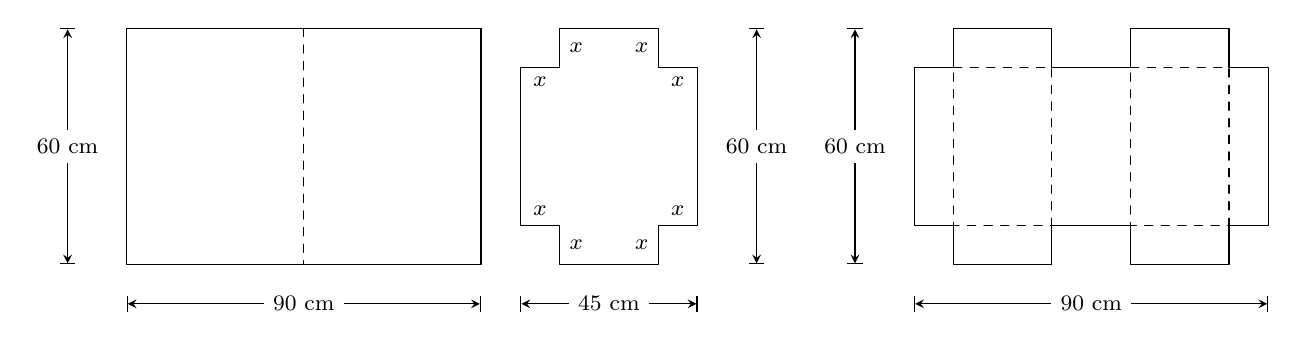
\begin{tikzpicture}[scale=1,>=stealth, font=\footnotesize, line join=round, line cap=round]
			\draw (0,0)--(4.5,0)--(4.5,-3)--(0,-3)--cycle;
			\draw[dashed] (2.25,0)--(2.25,-3);
			\draw (5,-0.5)--(5.5,-0.5)--(5.5,0)--(6.75,0)--(6.75,-0.5)--(7.25,-0.5)--(7.25,-2.5)--(6.75,-2.5)--(6.75,-3)--(5.5,-3)--(5.5,-2.5)--(5,-2.5)--cycle (5.25,-0.5)node[below]{$x$} (5.25,-2.5)node[above]{$x$} (7,-0.5)node[below]{$x$} (7,-2.5)node[above]{$x$} (5.5,-0.25)node[right]{$x$} (5.5,-2.75)node[right]{$x$} (6.75,-0.25)node[left]{$x$} (6.75,-2.75)node[left]{$x$};
			\draw[xshift=0.5cm] (9.5,-0.5)--(10,-0.5)--(10,0)--(11.25,0)--(11.25,-0.5)--(12.25,-0.5)--(12.25,0)--(13.5,0)--(13.5,-0.5)--(14,-0.5)--(14,-2.5)--(13.5,-2.5)--(13.5,-3)--(12.25,-3)--(12.25,-2.5)--(11.25,-2.5)--(11.25,-3)--(10,-3)--(10,-2.5)--(9.5,-2.5)--cycle;
			\draw[dashed,xshift=0.5cm] (10,-0.5)--(11.25,-0.5)--(11.25,-2.5)--(10,-2.5)--cycle (12.25,-0.5)--(13.5,-0.5)--(13.5,-2.5)--(12.25,-2.5)--cycle;
			\draw[|<->|] (-0.75,0)--(-0.75,-3) node[pos=.5,fill=white]{$60$ cm};
			\draw[|<->|] (8,0)--(8,-3) node[pos=.5,fill=white]{$60$ cm};
			\draw[|<->|] (9.25,0)--(9.25,-3) node[pos=.5,fill=white]{$60$ cm};
			\draw[|<->|] (0,-3.5)--(4.5,-3.5) node[pos=.5,fill=white]{$90$ cm};
			\draw[|<->|] (5,-3.5)--(7.25,-3.5) node[pos=.5,fill=white]{$45$ cm};
			\draw[|<->|] (10,-3.5)--(14.5,-3.5) node[pos=.5,fill=white]{$90$ cm};
		\end{tikzpicture}
	\end{center}
	\shortans[0]{$20{,}5$}
	\loigiai{
		Sau khi cắt bốn hình vuông cạnh $x, (0<x<\dfrac{45}{2})$ cm và gấp tấm bìa, kích thước của hình hộp là
		\begin{itemize}
			\item Chiều dài $60-2x$;
			\item Chiều rộng $45-2x$;
			\item Chiều cao $2x$.
		\end{itemize}    
		Thể tích khối hộp là
		\[
		V(x)=2x(60-2x)(45-2x)=8x^3-420x^2+5\,400x.
		\]
		Ta có $V'(x)=24x^2-840x+5400; V'(x)=0 \Leftrightarrow \hoac{
			&x=\dfrac{35+5\sqrt{13}}{2}\approx 36{,}18\,\,(\text{loại})\\
			&x=\dfrac{35-5\sqrt{13}}{2}\approx 13{,}82\,\,(\text{nhận}).
		}$\\
		Bảng biến thiên
		\begin{center}
			
\begin{tikzpicture}
				\tkzTabInit[nocadre,lgt=2.2,espcl=2.5,deltacl=0.5]
				{$x$/1.6,$V'(x)$/0.6,$V(x)$/2}
				{$0$,$\dfrac{35-5\sqrt{13}}{2}$,$\dfrac{45}{2}$}
				\tkzTabLine{,-,0,+,}
				\tkzTabVar{-/$ $,+/$V\left(\dfrac{35-5\sqrt{13}}{2}\right)$,-/$ $}
			\end{tikzpicture}
		\end{center}
		Vậy thể tích lớn nhất của khối hộp là $V\left(\dfrac{35-5\sqrt{13}}{2}\right)\approx 20\,468{,}04 \,\,\rm{cm^3}\approx 20{,}5$ lít.
	}
\end{ex}
\begin{ex}%Câu 6
	Trong không gian $Oxyz$, cho hai điểm $A(5;0;6)$ và $B(3;5;0)$. Điểm $M$ di động trên trục $Oz$, điểm $N$ di động trên trục $Oy$. Độ dài đường gấp khúc $AMNB$ có độ dài nhỏ nhất bằng bao nhiêu? (Kết quả làm tròn đến hàng phần chục).
	
	\shortans[0]{$13{,}5$}
	\loigiai{
		Để tìm độ dài ngắn nhất của đường gấp khúc $AMNB$ ta sẽ \lq\lq trải\rq\rq \, các điểm $A$, $B$ về cùng $1$ mặt phẳng $(Oyz)$ với các điểm $M$, $N$ và thoả mãn đoạn thẳng mới bằng với đoạn thẳng ban đầu (tức
		$AM=A'M; BM=BM'$) và đoạn gấp khúc ngắn nhất khi $4$ điểm trên thẳng hàng.\\
		Ta quay vuông góc mặt phẳng chứa điểm $A(5; 0; 6)$; (tức mặt phẳng màu xanh) xuống mặt phẳng $(Oyz$) ta được điểm $A'(0;-5; 6)$.\\
		Giả sử điểm $M(0; 0; z) \in Oz$. \\
		Suy ra $\heva{&AM=\sqrt{5^2+(z-6)^2}\\& A'M=\sqrt{(-5)^2+(z-6)^2}} \Rightarrow AM=A'M$.\\
		Tương tự, ta quay vuông góc mặt phẳng chứa điểm $B(3; 5; 0)$ (tức mặt phẳng màu hồng) xuống mặt phẳng $(Oyz)$ ta được điểm $B'(0;5;-3)$.\\
		Giả sử điểm $N(0; y; 0) \in Oy$. Suy ra $BN=BN'$.\\
		Ta có độ dài đường gấp khúc $AMNB=A'M+MN+NB'$.\\
		Suy ra $\left(AM'+MN+N'B\right)_{min}$ xảy ra khi $A'$, $M$, $N$, $B'$ thẳng hàng và bằng $A'B'$.
		\[A'B'=\sqrt{(5+5)^2+(-3-6)^2}=\sqrt{181}\approx 13{,}5.\]
	}
\end{ex}
\Closesolutionfile{ans}